\documentclass[10pt,conference]{IEEEtran}
\usepackage[dvipsnames]{xcolor}
\usepackage{standalone}
\usepackage{tikz}
\usepackage[utf8]{inputenc}
\usepackage[english]{babel}
\usepackage{booktabs}
\usepackage{tabu}
\usepackage[letterpaper]{geometry}
\usepackage[colorlinks]{hyperref}
\geometry{verbose,tmargin=2.5cm,bmargin=2.5cm,lmargin=2cm,rmargin=2cm,columnsep=0.8cm}
\usetikzlibrary{positioning, calc, shapes, fit, backgrounds, patterns}

\title{\textbf{Hardware accelerator topologies in heterogeneous systems: an evaluation in the
    security domain}}
\author{Bruno Morais}
\date{}

\begin{document}

\maketitle

\begin{abstract}
  Hardware accelerators (HWACCs) have driven performance gains for
  domain specific applications which leverage highly optimized computation
  cores. However, the traditional accelerator access topology as an add-on to
  general purpose processors through shared memory space/bus, reveals performance
  issues as the number of HWACCs grow and systems become
  communication-bound.
  On the other hand, efficient development and research of HWACCs
  that are closer to a general purpose processor's datapath is seen as a
  prohibitive task due to the required microarchitecture knowledge and lack of
  tools to explore the design space. This has in turn hindered the exploration of
  such architectures for gains in either performance or security spectrums.
  RISC-V projects made available in the last few years provide a framework that
  greatly eases microarchitecture research, enabling further experimentation
  into security and performance aspects for heterogeneous platforms.
  This work uses a customized RISC-V SoC to explore performance trade-offs
  between different HWACC topologies (in-datapath, memory-mapped) for embedded
  systems in the security domain by implementing an IP core for cryptographic
  primitive acceleration.
  % results also go in here

\end{abstract}

\section{Introduction}

\begin{figure}
  \centering
  \documentclass{standalone}
\usepackage[dvipsnames]{xcolor}
\usepackage{tikz}
\usetikzlibrary{positioning, calc, shapes, fit}

\begin{document}

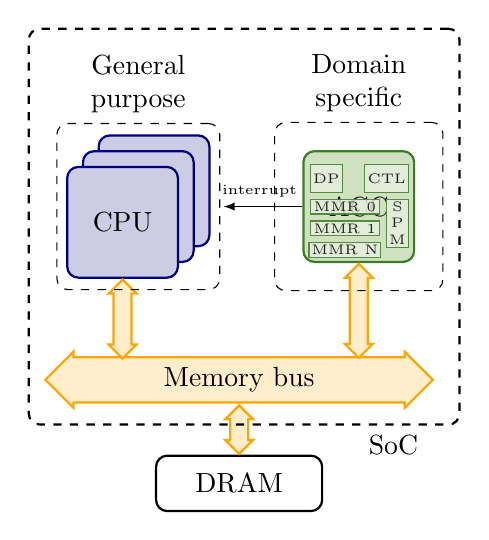
\begin{tikzpicture}
  \tikzstyle{PE}=[rounded corners, draw, thick, minimum size=40pt, align=center]
  \tikzstyle{core}=[PE, draw=NavyBlue, fill=NavyBlue!20]
  \tikzstyle{hwacc}=[PE, draw=OliveGreen, fill=OliveGreen!20]
  \tikzstyle{bus}=[double arrow, draw=Orange, fill=Orange!20, thick,
  minimum width=20pt, double arrow head extend=2pt]
  \tikzstyle{accint}=[draw=OliveGreen, fill=OliveGreen!10, outer sep=1pt, inner sep=1pt,
  node distance=0.5pt, opacity=0.85]

  \begin{scope}[name=soc, local bounding box=socbb]
  \node (core2) at (0.4,0.4) [core] {};
  \node (core1) at (0.2,0.2) [core] {};
  \node (core0) at (0,0) [core] {CPU};

  \node (hwacc1) at (3,0.2) [hwacc] {ACC};
  \begin{scope}[name=completeacc, local bounding box=accbb, shift={(3, 0.2)}]
    \node (reg0) [accint, minimum width=25pt, xshift=-5pt, minimum height=5pt, font=\tiny] {MMR 0};
    \node (reg1) [accint, minimum width=25pt, minimum height=5pt, below=of reg0, font=\tiny] {MMR 1};
    \node (reg2) [accint, minimum width=25pt, minimum height=5pt, below=of reg1, font=\tiny] {MMR N};
    \node (spm) [accint, minimum height=15pt, minimum width=5pt, align=center,
    right=of reg0.north east, font=\tiny, anchor=north west] {S\\P\\M};
    \node (accpe) [accint, minimum width=10pt, minimum height=10pt, above=of reg0.north west,
    anchor=south west, font=\tiny] {DP};
    \node (accctl) [accint, minimum width=10pt, minimum height=10pt, above=of spm.north east,
    anchor=south east, font=\tiny] {CTL};
  \end{scope}
  \node (mainbus) at (-1, -2) [bus, anchor=west, minimum height=140pt] {Memory bus};

  \node at (core0.south) [bus, rotate=90, anchor=east, scale=0.5, minimum height=57pt] {};
  \node at (hwacc1.south) [bus, rotate=90, anchor=east, scale=0.5, minimum height=68pt] {};

  \node (gpc) [fit=(core0)(core1)(core2), rounded corners,
  dashed, draw, minimum height=60pt, label={[align=center]90:{General\\ purpose}}] {};
  \node (dsc) [fit=(hwacc1), rounded corners, dashed, inner sep=10pt,
  draw, minimum height=60pt, label={[align=center]90:{Domain\\ specific}}] {};

  \draw[-latex] (hwacc1.west) -- ++(-1,0) node [anchor=south west, xshift=-4pt] {\tiny interrupt};
  \end{scope}

  \node (dram) [draw, rounded corners, below= of mainbus, minimum width=60pt,
  minimum height=20pt, yshift=10pt, thick] {DRAM};

  \node at (dram.north) [bus, rotate=-90, anchor=east, scale=0.5, minimum height=35pt] {};

  \node [fit=(socbb), draw, dashed, rounded corners, thick, inner sep=6pt, label={300:SoC}] {};

\end{tikzpicture}

\end{document}
  \caption{Loosely-coupled HWACCs: typical memory mapped HWACC usage in a heterogenous architecture.}
\end{figure}

\begin{figure}
  \centering
  \resizebox{0.3\textwidth}{!}{
    \begin{minipage}{0.5\textwidth}
      \centering
      \documentclass{standalone}
\usepackage[dvipsnames]{xcolor}
\usepackage{tikz}
\usetikzlibrary{positioning, calc, shapes, fit, backgrounds}

\begin{document}
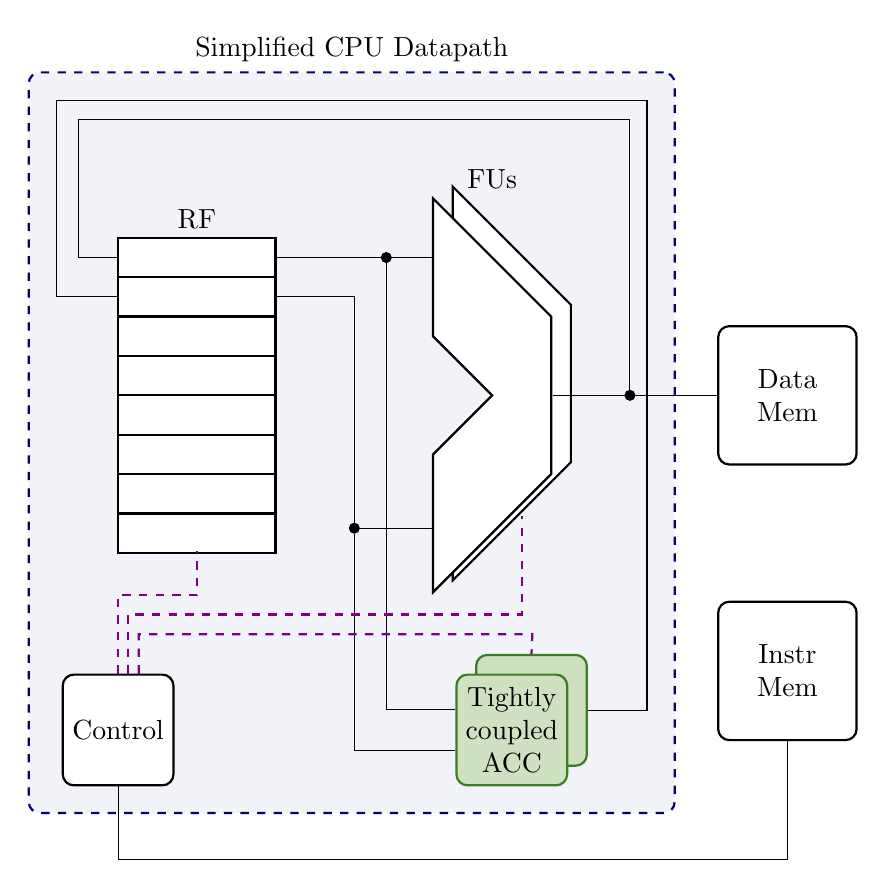
\begin{tikzpicture}
  \tikzstyle{coord}=[inner sep=0pt, outer sep=0pt, node distance=0pt]
  \tikzstyle{hwacc}=[rounded corners, draw=OliveGreen, fill=OliveGreen!20, thick, minimum size=40pt]
  \tikzstyle{control}=[draw=Purple, dashed, thick]
  \begin{scope}[name=datapath, local bounding box=dpathbb]

    % register file drawing
    \begin{scope}[name=rf, local bounding box=rfbb, shift={(0, -0.5)}]
      \node at (1,0) [anchor=south] {RF};
      \draw[fill=white, thick] (0,0) rectangle (2, -4);
      \foreach \i in {1,...,8} {
        \node (rfout\i) at (2, -0.5*\i+0.25) [coord] {};
        \node (rfin\i) at (0, -0.5*\i+0.25) [coord] {};
        \draw[thick] (0, -0.5*\i) -- (2, -0.5*\i);
      }
    \end{scope}

    % functional units
    \begin{scope}[name=fu, local bounding box=fubb, shift={(4, 0)}]
      \node at (0.75, 0) [anchor=south] {FUs};
      \begin{scope}[shift={(0.25, 0.15)}]
      \draw [fill=white, thick] (0, 0) -- (0, -1.75) -- (0.75, -2.5) -- (0, -3.25) -- (0, -5) -- (1.5, -3.5) -- (1.5, -1.5) -- cycle;
      \end{scope}
      \begin{scope}
        \draw [fill=white, thick] (0, 0) -- node [coord] (alua) {} (0, -1.75) -- (0.75, -2.5) -- (0, -3.25) -- node [coord] (alub) {}
        (0, -5) -- (1.5, -3.5) -- node [coord] (alux) {} (1.5, -1.5) -- cycle;
      \end{scope}
    \end{scope}

    % connections
    \draw (rfout1)  -| (alua);
    \draw (rfout2) -| ($(alub)!0.5!(rfout8)$) node (rfconn1) [coord, circle, fill=black, minimum size=4pt] {} -| (alub);
    \draw (alux) -- ++(1, 0) node (dataconn) [coord, circle, fill=black, minimum size=4pt] {} -- ++(0, 3.5) -- ++(-7, 0) |- (rfin1);

    % controller
    \node (ctl) at (0, -6.75) [draw, rectangle, rounded corners, minimum size=40pt, thick, fill=white] {Control};

    % tightly coupled acc
    \node (hwacc2) at (5.25, -6.5) [hwacc] {};
    \node (hwacc1) at (5, -6.75) [hwacc, align=center] {Tightly\\coupled\\ ACC};

    % accelerator connections
    \draw (hwacc2.east) -- ++(0.75, 0) -- ++(0, 7.75) -- ++(-7.5, 0) |- (rfin2);
    \draw (rfconn1) |- (hwacc1.200);
    \node (rfconn2) at (rfout1) [coord, circle, fill=black, minimum size=4pt, xshift=40] {};
    \draw (rfconn2) |- (hwacc1.160);
  \end{scope}

  \node (datamem) at (8.5, -2.5) [rounded corners, draw, thick, minimum size=50pt, align=center] {Data\\ Mem};
  \node (instmem) at (8.5, -6) [rounded corners, draw, thick, minimum size=50pt, align=center] {Instr\\ Mem};
  \draw (dataconn) -| (datamem.west);
  \draw (instmem.south) -- ++(0, -1.5) -| (ctl.south);

  % control lines
  \draw[control] (ctl.80) -- ++(0, 0.75) -- ++(5, 0) -- ++(0, 1.25);
  \draw[control] (ctl.90) -- ++(0, 1) -- ++(1, 0) -- ++(0, 0.55);
  \draw[control] (ctl.70) -- ++(0, 0.5) -- ++(1, 0);
  \draw[control] (ctl.70) -- ++(0, 0.5) -- ++(5, 0) -- (hwacc2.north);


  \begin{scope}[on background layer]
    \node [fit=(dpathbb), draw=NavyBlue, fill=NavyBlue!5, rounded corners, dashed, thick, inner sep=10pt,
    label={90:Simplified CPU Datapath}] {};
  \end{scope}
\end{tikzpicture}
\end{document}
    \end{minipage}
  }
  \caption{Tightly-coupled HWACCs: accelerator is moved into CPU datapath,
    operating similarly to microarchitectural Functional Units (FUs).}
\end{figure}

\section{Related work}

\subsection{Hardware accelerators?}
% Tightly vs loosely coupled hwaccs

\subsection{RISC-V instruction set extensions}
% Xcrypto

\section{Background}


\subsection{Embedded security: lightweight ciphers}

The industry standard ciphers might impose too much of a burden on deeply
embedded, low power systems that need the ability to communicate securely over
an unsecured channel. Thus, different organizations have hosted competitions to
foster the development of lightweight ciphers, targeting both resource-limited
software and hardware implementations.

In this evaluation, it is assumed that the object of study is such a system,
with strict area and power limitations. The Simon~\cite{Beaulieu2015} cipher family is chosen as a
lightweight cipher; it is a hardware-optimized cipher family developed by the
NSA. Although faced with controversies due to polarized views towards the
authors, it is an ISO standardized cipher.

The Simon family of ciphers offers different possibilities for both block and
key sizes. In all cases, both the round and key expansion functions make use
only of bitwise \texttt{XOR}, \texttt{AND}, and left and right circular shifts.
Figure~\ref{fig:simonround} shows the Feistel stepping of its round function.

\begin{figure}
  \centering
  \documentclass{standalone}
\usepackage[dvipsnames]{xcolor}
\usepackage{tikz}
\usetikzlibrary{positioning, calc, shapes, fit, backgrounds, patterns}

\begin{document}
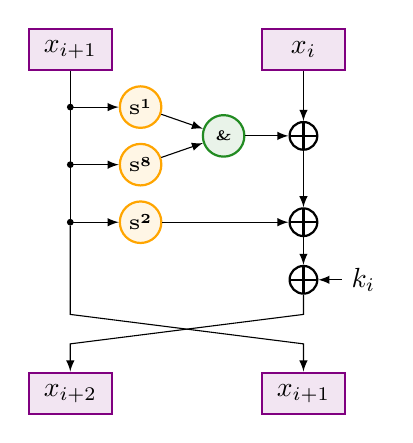
\begin{tikzpicture}
\tikzstyle{roundblock}=[draw=Purple, thick, fill=Purple!10, minimum width=30pt, minimum height=15pt]
\tikzstyle{function}=[draw=Orange, circle, thick, fill=Orange!10, minimum size=15pt,
font=\tiny\bfseries, node distance=5pt, inner sep=0pt]
\tikzstyle{XOR}=[draw,circle, minimum size=10pt, thick, append after command={
      [shorten >=\pgflinewidth, shorten <=\pgflinewidth,]
      (\tikzlastnode.north) edge[thick] (\tikzlastnode.south)
      (\tikzlastnode.east) edge[thick] (\tikzlastnode.west)},
    node distance=10pt]
\tikzstyle{junct}=[inner sep=0pt, circle, draw, fill=black, minimum size=2pt]

% inputs
\node (inpx) [roundblock] {$x_{i+1}$};
\node (inpy) [roundblock, right=of inpx, xshift=25pt] {$x_i$};

% shifts
\node (s1) [function, below=of inpx.south east, xshift=10pt] {S\textsuperscript{1}};
\node (s8) [function, below=of s1] {S\textsuperscript{8}};
\node (s2) [function, below=of s8] {S\textsuperscript{2}};

% and
\node (and) at ($(s1)!0.5!(s8)$) [function, draw=ForestGreen, fill=ForestGreen!10, xshift=30pt] {\&};

% xors
\node (xor1) at (and -| inpy) [XOR] {};
\node (xor2) at (s2 -| xor1) [XOR] {};
\node (xor3) [XOR, below=of xor2] {};

\node (key) [right=of xor3, xshift=-20pt] {$k_i$};

% connections
\draw[-latex] (s1) -- (and);
\draw[-latex] (s8) -- (and);
\draw[-latex] (and) -- (xor1);
\draw[-latex] (s2) -- (xor2);
\draw[-latex] (inpy) -- (xor1);
\draw[-latex] (xor1) -- (xor2);
\draw[-latex] (xor2) -- (xor3);
\draw[-latex] (inpx.south) |- node (junct1) [junct] {} (s1);
\draw[-latex] (junct1) |- node (junct2) [junct] {} (s8);
\draw[-latex] (junct2) |- node (junct3) [junct] {} (s2);
\draw[-latex] (key) -- (xor3);

% out
\node (outx) [roundblock,  below=of inpx, yshift=-80pt] {$x_{i+2}$};
\node (outy) [roundblock, right=of outx, xshift=25pt] {$x_{i+1}$};

\draw[-latex] (xor3.south) -- ++(0, -0.25) node (coord1) {} -- ([yshift=10pt]outx.north) -- (outx.north);
\draw[-latex] (junct3) -- (coord1 -| junct3) -- ([yshift=10pt]outy.north) -- (outy.north);


\end{tikzpicture}
\end{document}

  \caption{Simon's round function Feistel stepping. \textbf{S\textsuperscript{j}} are
    circular left shifts by j bits; \textbf{\&} is a bitwise \texttt{AND}
    operation and $\oplus$ are bitwise \texttt{XOR} operations.}
  \label{fig:simonround}
\end{figure}

The number of necessary rounds is determined by the configuration of the cipher.
In this work we explore only the Simon64/128 and Simon128/128 configurations,
which require a number of 44 and 68 rounds per block, respectively.
In the nomenclature Simon\textbf{N}/\textbf{M}, \textbf{N} is the block size and
\textbf{M} is the key size in bits.

\subsection{RISC-V ecosystem}

The RISC-V ecosystem is rapidly growing, with many different implementations of
the RISC-V ISA standard currently available online. The complete GNU toolchain
is also available for the architecture and its standard extensions.

There are several alternatives in order to assemble a complete System on Chip
(SoC) for experimentation or synthesis purposes. Several different vendors /
open source community-provided designs can be used to kickstart development.

To assemble an entire SoC for cycle-accurate simulation, UC Berkeley's Chipyard~\cite{Chipyard}
is chosen.

\begin{figure}
  \centering
  \resizebox{0.45\textwidth}{!}{
    \begin{minipage}{0.5\textwidth}
      \centering
      
\documentclass{standalone}
\usepackage[dvipsnames]{xcolor}
\usepackage{tikz}
\usetikzlibrary{positioning, calc, shapes, fit, backgrounds, patterns}

\begin{document}
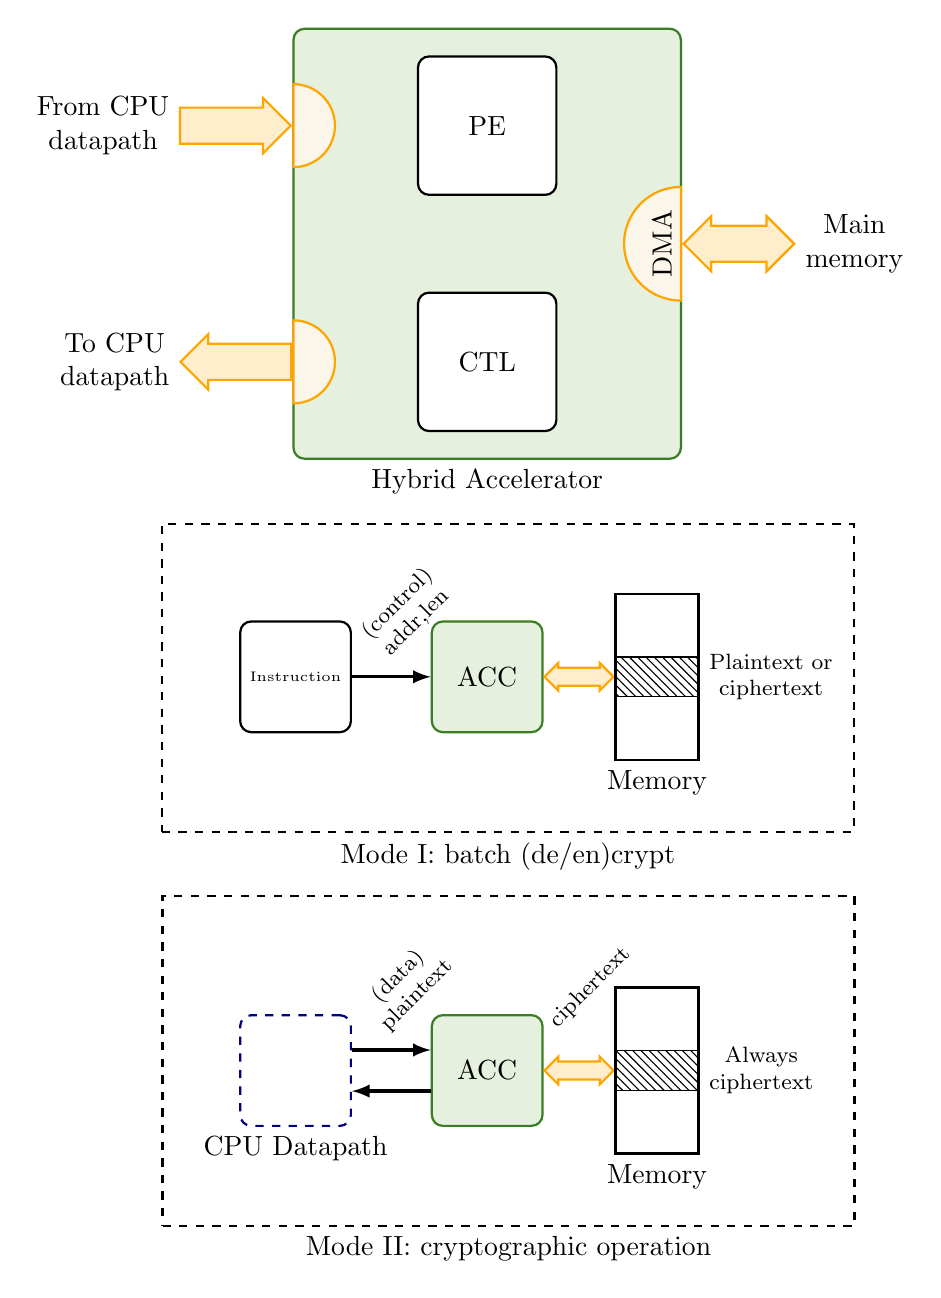
\begin{tikzpicture}
  \tikzstyle{accelement}=[rounded corners, draw, thick, minimum size=50pt, fill=white]
  \tikzstyle{port}=[semicircle, draw=Orange, fill=Goldenrod!10, anchor=south, thick]
  \tikzstyle{bibus}=[double arrow, draw=Orange, fill=Orange!20, thick,
  minimum width=20pt, double arrow head extend=2pt]
  \tikzstyle{ibus}=[single arrow, draw=Orange, fill=Orange!20, thick,
  minimum width=20pt, single arrow head extend=2pt]
  \tikzstyle{obus}=[single arrow, draw=Orange, fill=Orange!20, thick,
  minimum width=20pt, single arrow head extend=2pt, rotate=180]
  \tikzstyle{hwacc}=[rounded corners, draw=OliveGreen, fill=OliveGreen!10, thick]

  \begin{scope}[name=accstruct]
    \begin{scope}[name=acc, local bounding box=accbb]
      \node (accpe) [accelement] {PE};
      \node (accctl) at (0, -3) [accelement] {CTL};
    \end{scope}

    \begin{scope}[on background layer]
      \node (acc) [hwacc, fit=(accbb),
      minimum width=140pt, inner sep=10pt, label={270:Hybrid Accelerator}] {};
    \end{scope}

    \node (dmaport) at (acc.east) [port, minimum height=20pt, align=center,
    rotate=90] {DMA};
    \node (pathin) at (acc.west |- accpe.west) [port, rotate=270, anchor=south,
    minimum height=15pt] {};
    \node (pathout) at (acc.west |- accctl.west) [port, rotate=270, anchor=south,
    minimum height=15pt] {};

    \node (memconn) [bibus, anchor=west, minimum height=40pt, label={[align=center]0:{Main\\memory}}] at (dmaport.south) {};
    \node (fromdp) [ibus, anchor=east, minimum height=40pt, label={[align=center]180:{From CPU\\datapath}}] at (pathin.south) {};
    \node (todp) [obus, anchor=west, minimum height=40pt, label={[align=center]0:{To CPU\\datapath}}] at (pathout.south) {};
  \end{scope}

  \begin{scope}[name=op1, shift={(0, -7)}, local bounding box=mode1bb]
    \node (acc1) [hwacc, minimum size=40pt] {ACC};
    \node (inst) [draw, thick, rounded corners, left=of acc1, minimum size=40pt] {\tiny Instruction};
    \draw[-latex, very thick] (inst) -- node [anchor=south west, rotate=45, font=\footnotesize, align=center] {(control)\\addr,len} (acc1);
    \node (mconn1) at (acc1.east) [bibus, scale=0.5, anchor=west, minimum height=50pt] {};
    \node (dram1) at (mconn1.east) [draw, thick, minimum width=30pt, minimum height=60pt, anchor=west, label={270:Memory}] {};
    \draw [pattern=north west lines] (dram1.155) rectangle (dram1.335);
    \node at (dram1.east) [anchor=west, align=center, font=\footnotesize] {Plaintext or\\ciphertext};
  \end{scope}

  \node [draw,dashed, thick, fit=(mode1bb), inner sep=10pt, minimum width=250pt, label={270:Mode I: batch (de/en)crypt}, xshift=-12pt] {};

  \begin{scope}[name=op2, shift={(0, -12)}, local bounding box=mode2bb]
    \node (acc2) [hwacc, minimum size=40pt] {ACC};
    \node (dp) [draw=NavyBlue, thick, dashed, rounded corners, left=of acc2, minimum size=40pt, label={270:CPU Datapath}] {};
    \draw[-latex, very thick] (dp.20) -- node [anchor=south west, rotate=45, align=center, font=\footnotesize] {(data)\\plaintext} (dp.20 -| acc2.west);
    \draw[-latex, very thick] (dp.340 -| acc2.west) -- (dp.340);
    \node (mconn2) at (acc2.east) [bibus, scale=0.5, anchor=west, minimum height=50pt] {};
    \node (dram2) at (mconn2.east) [draw, thick, minimum width=30pt, minimum height=60pt, anchor=west, label={270:Memory}] {};
    \draw [pattern=north west lines] (dram2.155) rectangle (dram2.335);
    \node at (dram2.east) [anchor=west, align=center, font=\footnotesize] {Always\\ciphertext};
    \node at ([shift={(4pt, 30pt)}]mconn2) [align=center, rotate=45, font=\footnotesize] {ciphertext};
  \end{scope}

  \node [draw,dashed, thick, fit=(mode2bb), inner sep=10pt, minimum width=250pt,  label={270:Mode II: cryptographic operation}] {};

\end{tikzpicture}
\end{document}

    \end{minipage}
  }
  \caption{Hybrid crypto HWACCs: \textbf{upper}: HWACC is directly accessible through CPU datapath and
    integrated with memory hierarchy; \textbf{lower}: two operation modes; I: batch
    background processing of memory region (CPU not taxed); II: cryptographic
    operation where plaintext is only visible inside CPU datapath.}
  \label{fig:hybrid}
\end{figure}

\section{The Hybrid Crypto Accelerator}

Going one step further than the two previously discussed topologies used for
accelerators, we present a slightly different hybrid approach which has
some interesting characteristics. Figure~\ref{fig:hybrid} shows the concept and
possible operation modes of the hybrid crypto accelerator.

The hybrid crypto accelerator is distinct from the tightly-coupled topology in
the way that it has a DMA port for direct access to the coherent memory
hierarchy. This allows the accelerator to directly request data to be loaded and
stored, enabling two different modes of operation.

\subsection{Operation mode I: batch processing}

In this operation mode, specific instructions configure the accelerator to
batch perform encryption or decryption over a memory region. The accelerator
then proceeds to work while the CPU is left free for any other tasks that might
be waiting for CPU time.


\subsection{Operation mode II: cryptographic operation}

Differently from mode I, this mode allows for operation in the security domain,
isolating plaintext and ciphertext completely in the CPU datapath and memory.

In this mode, data is moved to/from memory by the CPU, through the accelerator,
which transparently encrypts or decrypts the data stored/loaded. Note that in
this mode, actual data (words) in the CPU datapath is passed in/out of the
accelerator, not control (load/store).

\section{Experimental setup}

In order to understand the area and performance trade-offs between the usage of
different system topologies, both a reference software implementation and an IP
core that performs the Simon cipher are implemented and tested on a RISC-V core.

The first step is to verify basic functionality by means of functional simulations.

\subsection{Functional simulation}

Functional simulation is accomplished with Spike~\cite{spike}, which is a RISC-V
instruction set simulator. Spike allows for execution of riscv64 binaries, and
also allows for implementation of C++ extensions that emulate the
functionalities of both memory-mapped peripherals and RoCC accelerators. Both
extensions are implemented to emulate functionality of different Simon
accelerators, and checked for result correctness against the reference software
implementation.


\subsection{Simon HWACCs}

After the functional simulations are performed with correct results, the Simon
cipher IP core was implemented in Chisel~\cite{chisel}. This was a necessary
choice since the infrastructure used to build the SoC to be evaluated is
completely built using Chisel.

The core Simon cipher functionality is implemented as the core IP and is
re-utilized to build three different accelerator types: memory-mapped
(loosely-coupled), RoCC (tightly-coupled and hybrid). In essence the the
accelerators are built by constructing wrappers around the common core.

The first two accelerators have similar functionality: the user must initialize the
accelerator by storing a key, at which point the acelerator core performs
necessary key expansion and waits for input data that is to be
encrypted/decrypted. Those accelerators support two different Simon widths:
Simon64/128 and Simon128/128.

The memory-mapped accelerator can operate in two different ways: i) automatic
operation --- ECB mode only, in which all necessary rounds are performed over a word until
completion of encryption/decryption process, or ii) interactive or single operation, where
software issues one round at a time, which enables software implementation of
CBC or other modes.

The tightly-coupled accelerator only operates interactively; that is, the
software manually issues an instruction that computes a round repetitively
until the complete process is done; encryption modes are thus
implemented in software.

The hybrid accelerator also needs to be initialized with a key. However, due to
development constraints, the accelerator only supports Simon64/128 in ECB mode.


\subsection{Full-scale SoC simulation}

Chipyard is used to generate synthesizable Verilog for the
entire SoC, including RISC-V CPU core and accelerators under test. The tool also
contains the necessary scripts to produce a cycle-accurate simulation of the
SoC, compiled with Verilator. After configuration of the environment, the Simon
chisel implementation is integrated in the SoC.

In Chipyard the option of either building the SoC using in-order (Rocket) or
out-of-order (BOOM) cores is given to the user. SoCs are built using both
alternatives for evaluation.

\subsection{Synthesis metrics}

Unfortunately, while the output from Chipyard is indeed synthesizable Verilog,
no support for targeting FPGA boards is readily available. Instead, the focus of
the tool is to enable VLSI flows for taping out custom ASICs.

However, Chipyard shares much of common RISC-V infrastructure that is maintained
by the CHIPS Alliance, it is possible to modify other projects that also use the
same infrastructure, and do target FPGA boards to include our accelerators. This
flow is used mainly for area evaluation purposes and not fully concerned with
actually running code on an FPGA prototyping target. SiFive's Freedom Platform
dev kit is chosen for this task.

\section{Evaluation results}

\subsection{Performance}

\begin{figure}
  \centering
  \includegraphics[width=\linewidth]{media/ecb_speedup}
  \caption{Speedup using different accelerator configurations in ECB mode.
    Values are relative to the in-order pure software implementation.}
  \label{fig:ecbspeedup}
\end{figure}

\begin{figure}
  \centering
  \includegraphics[width=\linewidth]{media/cbc_speedup}
  \caption{Speedup using different accelerator configurations in CBC mode.}
  \label{fig:cbcspeedup}
\end{figure}

To evaluate performance, we consider the case where a plaintext block with a size of
1 kB is encrypted using different implementations of the Simon cipher, yielding
eight different benchmarks:

\begin{itemize}
\item Pure software: ECB and CBC mode
\item MMIO accelerator, single: ECB and CBC mode
\item MMIO accelerator, automatic: ECB mode
\item Tightly-coupled accelerator: ECB and CBC mode
\item Hybrid accelerator: ECB mode
\end{itemize}

Usage of the MMIO accelerator in automatic mode highlights the characteristics
of a heterogeneous system that is computation-bound, whereas usage of it in the
single mode intends to model a communication-bound architecture.

The reference software implementation is used as a baseline,
Figures~\ref{fig:ecbspeedup},\ref{fig:cbcspeedup} show the relative speedup
(computed from the total cycle count for each of the benchmarks) of alternative
implementations using accelerators or a 2-way BOOM core for encryption in ECB
and CBC mode, respectively.

% TODO small interpretation paragraph here

\begin{figure}
  \centering
  \includegraphics[width=\linewidth]{media/scatter_results}
  \caption{Distribution of all benchmark results with respect to both total
    number of instructions retired by processor and total number of cycles
    required to complete operations.}
  \label{fig:scatter}
\end{figure}

\subsection{Area}

\subsection{Security implications}

It is of note that while this work implements a cryptographic primitive that can
be used in-hardware to enable acceleration of ciphers, it is a proof-of-concept
level rudimentary implementation.

Under more critical scrutiny there would be a few immediately reconizeable
issues:

\begin{itemize}
  \item In some configurations, accelerators can only perform in ECB mode in
    hardware, limiting both security and performance. To overcome this, the
    accelerator implementation needs to be extended to be more flexible/complex
    and include such operation modes.
  \item Due to the use of generic instruction / RoCC interface, accelerators
    can be exploited by attacker at unprivileged level. To overcome this,
    accelerators and toolchain must be modified to use customized instructions,
    which can be configured for certain privilege levels only
\end{itemize}

\section{Future work}

As future work, there is much room for improvement; better understanding of how
to leverage the memory coherence hierarchy in the hybrid accelerator model
should lead to better performance; accelerator can be developed further to
accept more encryption modes, including parallelization; security can be
hardened by enforcing privilege levels at the hardware level, to name a few.

Also, a set of different, reutilizable cryptographic primitives can be further
explored and integrated into a larger multi-accelerator framework for
acceleration of other demanded cryptographic functions such as hash functions
and possible compositions of primitives for message authentication, for instance.

These require a more thorough and complex modification of the available
toolchain and datapath microarchitecture, as it is likely that the standard RoCC
interface will not be able to provide the desired flexibility and control
granularity levels for detailed exploration.

\section{Conclusions}

\bibliography{paper}
\bibliographystyle{ieeetr}

\end{document}